{
    \renewcommand*{\theenumi}{\thesubsection.\arabic{enumi}}
    \renewcommand*{\theenumii}{\theenumi.\arabic{enumii}}
    \renewcommand*{\theenumiii}{\theenumii.\arabic{enumiii}}

    \section{Software Architecture}

    \subsection{Website}

        The website will be created using Django and Python. It will be hosted 
        on an Apache server. The front end will use HTML, CSS, and Javascript
        to create the viewed website.

        The reason for using Django is that it is flexible and allows for 
        a multitude of plugins to use. It also allows for a website to be built
        quickly without compromising quality. It is open source which allows
        for free use and can be changed if need be.

        Django gives an easy-to-use database interface. It creates the databse,
        along with sanitizing all SQL queries and ensure than any user input
        is escaped preventing XSS. 

    \subsection{Android App}
        
        The Android app will be written in Android Java and XML to be a native
        app. The app will communicate with the back end server in the same 
        manner as the website. 

    \subsection{Apache Server}

        The Apache server will host the Django website and send the site over
        port 80 to the client.

        \begin{figure}[htb]
            \centering
            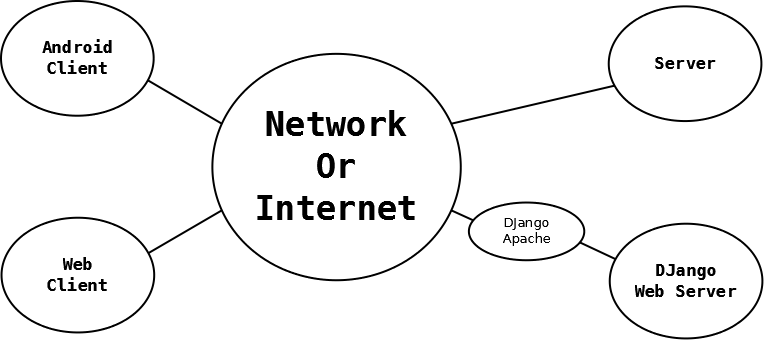
\includegraphics[width=0.9\textwidth]{Images/Web.png}
            \caption{Diagram showing server and client connections}
            \label{fig:NetworkDiagram}
        \end{figure}
    
    \subsection{PostgreSQL}

        The PostgreSQL database will store login credentials, drinks, and list
        of drinks saved for each user. All private or sensitive information 
        stored in the database will be salted and hashed before being put into 
        the server.
}
